\documentclass[english]{ccdconf}
\usepackage{amsmath}
\usepackage{subfigure}
\graphicspath{{image/}}
\begin{document}


\title{3D Object Detection in RGBD Image Using View Independent Feature}
\author{Jiang Liu\aref{sjtu}, Jianxun Li\aref{sjtu2}}

\affiliation[sjtu]{School of Electronic Information and Electrical Engineering,
Shanghai Jiao Tong University, Shanghai, 200240
        \email{jiangliux@sjtu.edu.cn}}


\affiliation[sjtu2]{School of Electronic Information and Electrical Engineering,
	Shanghai Jiao Tong University, Shanghai, 200240
	\email{lijx@sjtu.edu.cn}}

\maketitle

\begin{abstract}
These instructions give you basic guidelines for preparing papers
for Chinese Control and Decision Conference . Note that ``Abstract''
and ``Key Words'' are bold.
\end{abstract}

\keywords{Paper, Instruction, Chinese Control and Decision
Conference }

\section{INTRODUCTION}

3D object detection has received considerable attention recently for the wide range of applications in autonomous driving and personal robotics\cite{xiang2014beyond}. Traditional detection method only localize objects in 2D bounding boxes, missing the information of 3D location, orientation and 3D extent. In contrast, 3D object detection provide accurate 3D information to understand real world, thus plays an important role in morden computer vision.\\
It is difficult to solve this task in RGB image due to its natrual ambiguity of missing depth. The most common approach is to discretize the viewing sphere into bins and train a 2D detector for each viewpoint \cite{gu2010discriminative}. However, only weak 3D information can be obtained in these methods. Besides, object-centerd methods establishes spatial connections betwee views by mapping them directly to the surface of 3D model. Though these types of models seems attractive for the continuous viewpoint represantations, their detection performance has typically been inferior to 2D deformable models. More recently, \cite{fidler20123d} extend 2D deformable part-based models(DPMs)\cite{felzenszwalb2010object} to 3D space by means of a deformable 3D cuboid.\\
With the the availability of inexpensive RGB-D sensors, such as Microsoft Kinect, Apple PrimeSense, Intel RealSense, and Google Project Tango, larger and more ambitious RGBD datasets are created which enabled major breakthroughs for highlevel scene understanding\cite{silberman2012indoor,janoch2013category}. SUN RGB-D dataset\cite{song2015sun}, which contains 10,335 RGB-D images with dense annotations in 3D, has become a de-facto standard for scene understanding.\\
It is important to exploit the depth information to advance 3D object detection. Sliding Shapes\cite{song2014sliding} was proposed to slide a 3D detection window in 3D space, detect objects by matching to CAD models in “sliding” locations. While CAD models can potentially provide abundant information, the number of models for all categories is limited, and thus this method focused only on a small number of categories. Ren\cite{ren2016three} proposed the Clouds of Oriented Gradients(COG) feature that links the 2D appearance and 3D pose of object categories. COG accurately describes the 3D appearance of objects with complex 3D geometry.\\
We improved 3D object deteion algorithm based on \cite{ren2016three}. Our contribution are mainly two folds:
first, Instead of scanning every possible location and orientation in 3D space, we use rectified 3D Selective Search to dramaticlly speed up the testing process with a relative high recall. 
second, object pruning is uesed to reduce candidate object hypothesis in testing stage, thus reduce testing time as well as false positive detection.
\begin{figure}
	\centering
		\subfigure[RGB Image]{
			\includegraphics[width=0.47\hsize]{1/53o.eps}
			\label{image1-1}
		}
		\subfigure[Depth Image]{
		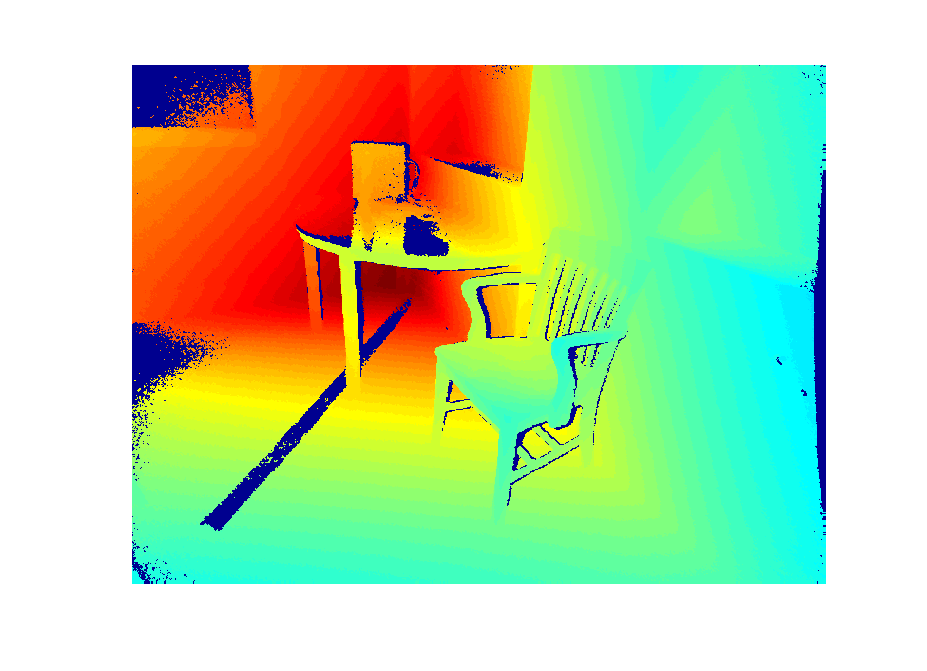
\includegraphics[width=0.47\hsize]{1/53d.eps}
		\label{image1-2}
		}
	
	\subfigure[Detection Result]{
		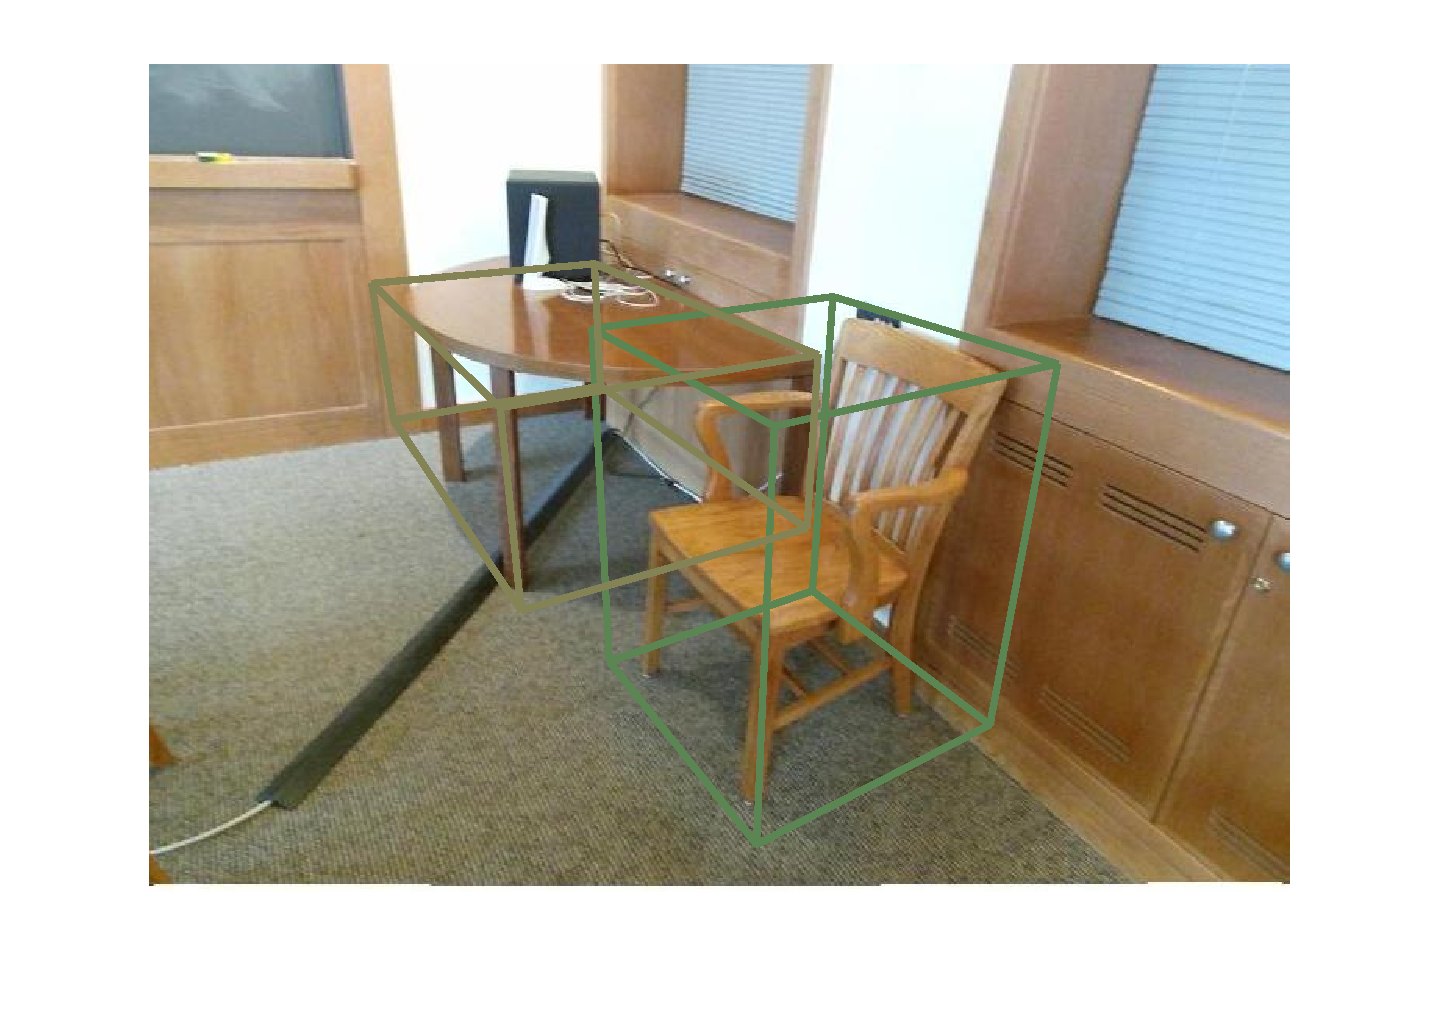
\includegraphics[width=0.47\hsize]{1/53c.eps}
		\label{image1-3}
	}
	\subfigure[Detection Result]{
		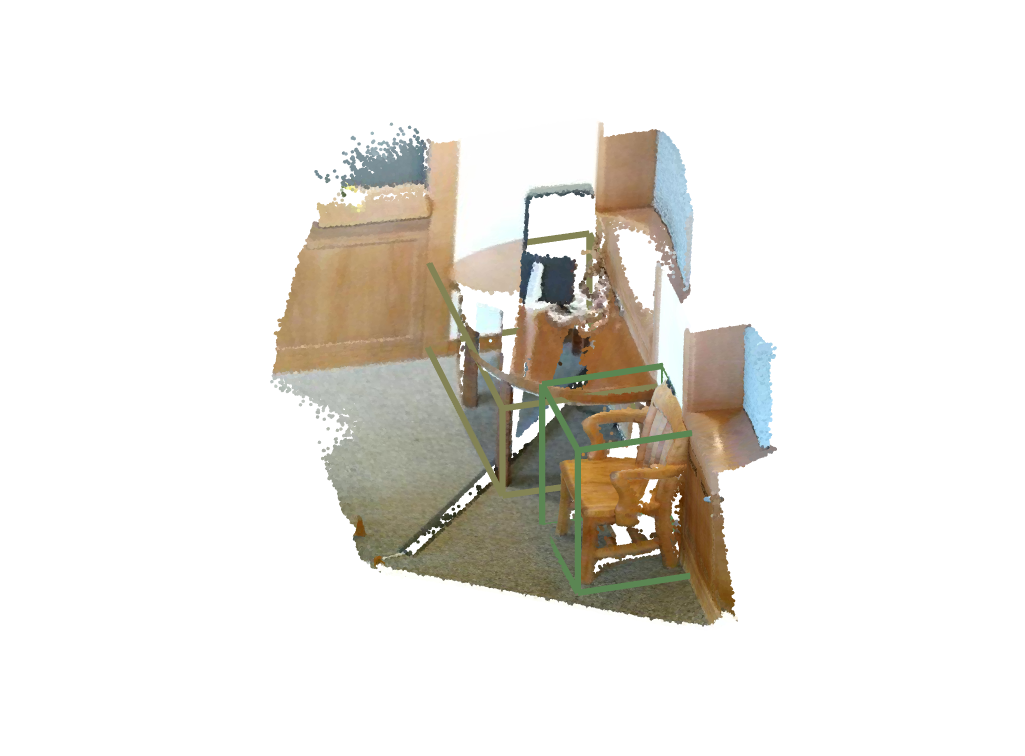
\includegraphics[width=0.47\hsize]{1/53.eps}
		\label{image1-4}
	}
	\caption{A illustrative example define the task of 3D object detection. Top row are the RGB image and depth image of same scene from SUN RGBD dataset. Given them as input, we need to find out the cuboid containing the objects of interst. \ref{image1-3} is the detection result in projected RGB image while \ref{image1-4} display them in 3D.}
	\label{pipeline}
\end{figure}
\section{Related Work}

\subsection{3D Feature}
\label{3D Feature}
The histogram of oriented gradient (HOG) descriptor \cite{dalal2005histograms} is widely used in object detection. Basiclly, it counts occurrences of gradient orientation in localized portions of an image, and its performance is good enough for 2D detection.  However, since gradient orientations are determined by 3D object orientation and perspective projection, HOG descriptors that are naively extracted in 2D image coordinates is not suitable for 3D object description.\\
%To handle this issue, The cloud of oriented gradient(COG) feature, without all these assumption, accurately model the 3D apperence of objects.\\
To handle this issue,  many work has been done. some used extra CAD model to describe the edge from various viewpoints\cite{aubry2014seeing}.Other assumed that object in sepecific views are near-planar\cite{fidler20123d}. previous extensions of the HOG descriptor  to 3D space require full mesh model\cite{buch20093d}. Rencently the cloud of oriented gradient(COG) feature\cite{ren2016three} is proposed to accurately model the 3D apperence of objects. Like HOG , the calculation of COG can be divided into 3 step: Gradient computation, 3D orientation bin construction and normalization. In the first step, gradient of the image is computed by applying filters [-1,0,1], [-1,0,1]$^\mathrm{T}$ to RGB channels. Gradient in position $(x,y)$ is obtained by setting  maximum responses across
color channels to $(dx,dy)$, with corresponding magnitude $\sqrt{(dx^2+dy^2)}$.
Then, cuboid contains the object is devided it into $6\times6\times6$ voxels, and 9 orientation bins are constructed for each voxel to model the distribution of local 3D gradient orientation. Perspective projection is used to find corresponding 2D bin boundaries. For each point lies in a voxel, its projected gradient magnitude is sumed into corresponding 2D orientation bin, which is back-projected into 3D bin. Last, bilinearly interpolation is performed between neighboring bins.
 Histogram $\phi_{il}^a$for voxel $l$ in cuboid $i$ is normalized by setting $\phi_{il}^a \leftarrow \phi_{il}^a / \sqrt{\|\phi_{il}^a \|^2+ \epsilon}$ for a small $\epsilon>0$, so the dimension of COG feature is a fixed size of $6^3\times9=1944$.\\
 Besides the apperance features like COG, other 3D features aim to model the object geometry like point cloud density and 3D normal orientation. For voxel $l$ in cuboid $i$ contains $N_{il}$ points, the point cloud density feature equals $\phi_{il}^b=N_{il}/A_{il}$, where $A_{il}$ is the are of silhoutte of the voxel. This kind of normalization makes the object in the scene robust to depth variation and partial occlusion. 3D normal orientation feature $\phi_{il}^c$ is obtained by building a 25-bin histogram of normal orientation within voxel $l$. The normnal orientation of each 3D point is calculated via a plane fit to its some nearest neighbors. These geometry features combined with appearence features are able to most accurately model the object in 3D.
\subsection{3D Search}
\label{3D Search}
Search algorithm define the hypothesis space for potention object location in testing image. Sliding window method is widely used in 2D detection algorithm\cite{dalal2005histograms,felzenszwalb2010object} and the core idea is intuitive.  An exhaustive search with predefined step is performed where all the location within the image is scanned to not miss any potential object location. Scale is considered by examined different size of image patch at that location. However, searching all the possible location is computationally expensive. Selective search is proposed for fast computation with high recall\cite{uijlings2013selective}. First, initial regions is obtained by performing fast segmentation\cite{felzenszwalb2004efficient}. Later, the most similar neighbouring region pair is merged into a new region and add to the set in every iteration. Finally, object location boxes are extracted from all regions in the set.\\
The current search methods in 3D naively generlized from 2D. Sliding shape\cite{song2014sliding} train an Exemplar-SVM on a CG model rendered at a specific 3D location relative to the virtual camera, then perform exhaust search only at the nearby location of the CG model in order to improve the speed. This 3D local search approach results a relative low recall rate. In \cite{ren2016three}, 3D space is discritized into grids. The at each possible location, certain size of bounding boxes which based on the empirical statistics of trainning bounding boxes, along with 16 candidate orientation are examined. This strategy brings a high recall rate but introduce many false positive detection.\\
3D selective search(3D SS) is first  proposed in \cite{kanezaki20153d}. But it finally outputs candidate bounding boxes in 2D image. \cite{song2016deep} rectified this method and output 3D bounding boxes. First, RANSAC is used to fit the pane of 3D point cloud to obtain an initial segmentation. For each plane that its projection covers more than 10\% of the total image area,
RGB-D UCM segmentation from \cite{gupta2014learning}(with threshold 0.2) is used for further splitting. Then starting with this oversegmentation, different segmentation regions are hierarchically grouped, with the following similarity measures:
\begin{itemize}
\item $s_{color}(r_i,r_j)$ is the measurment of color similarity between region $r_i$ and $r_j$ using RGB color histogram intersection.
\item $s_{\#pixels}(r_i,r_j)=1-\frac{\#pixels(r_i)+\#pixels(r_j)}{\#pixels(im)}$, where $\#pixels(\cdot)$ is number of pixels in this region.
\item
$s_{volume}(r_i,r_j)=1-\frac{volume(r_i)+volume(r_j)}{volume(room)}$, where $volume(\cdot)$ is the volume of 3D bounding boxes of the points in this region.
\item
$s_{fill}(r_i,r_j)=1-\frac{volume(r_i)+volume(r_j)}{volume(r_i \cup r_j)}$ describe how well region $r_i$ and $r_j$ fit into each other.
\end{itemize}
The weighted sum of these four terms form the final output of similarity measuremenmt. Since both 3D and color cues are combined,
this very strong baseline achieves an average recall 74.2. However, for convinience, orientations of all the cuboid are the same with room orientation, which reduce the accuracy of detection.\\.
\section{PIPELINE}
Our whole pipeline is shown in Fig \ref{pipeline}. During trainning(Sec. \ref{Train}), we learn a structred SVM for each class with COG combined with geometry features described in Sec. \ref{3D Feature}, without the extra information of CG model. During testing(Sec. \ref{Test}), we use learned structured SVMs to classify candidate cuboids , and output 3D bounding boxes with detection scores.\\
Instead of exhuastively searching testing image as in \cite{ren2016three}, we speed up testing step dramaticlly with few loss of recall using 3D SS. With object pruning, we further reduce the testing time by saving time for feature computing, and reduce false positive without much recall decrease.
\begin{figure}
  \centering
  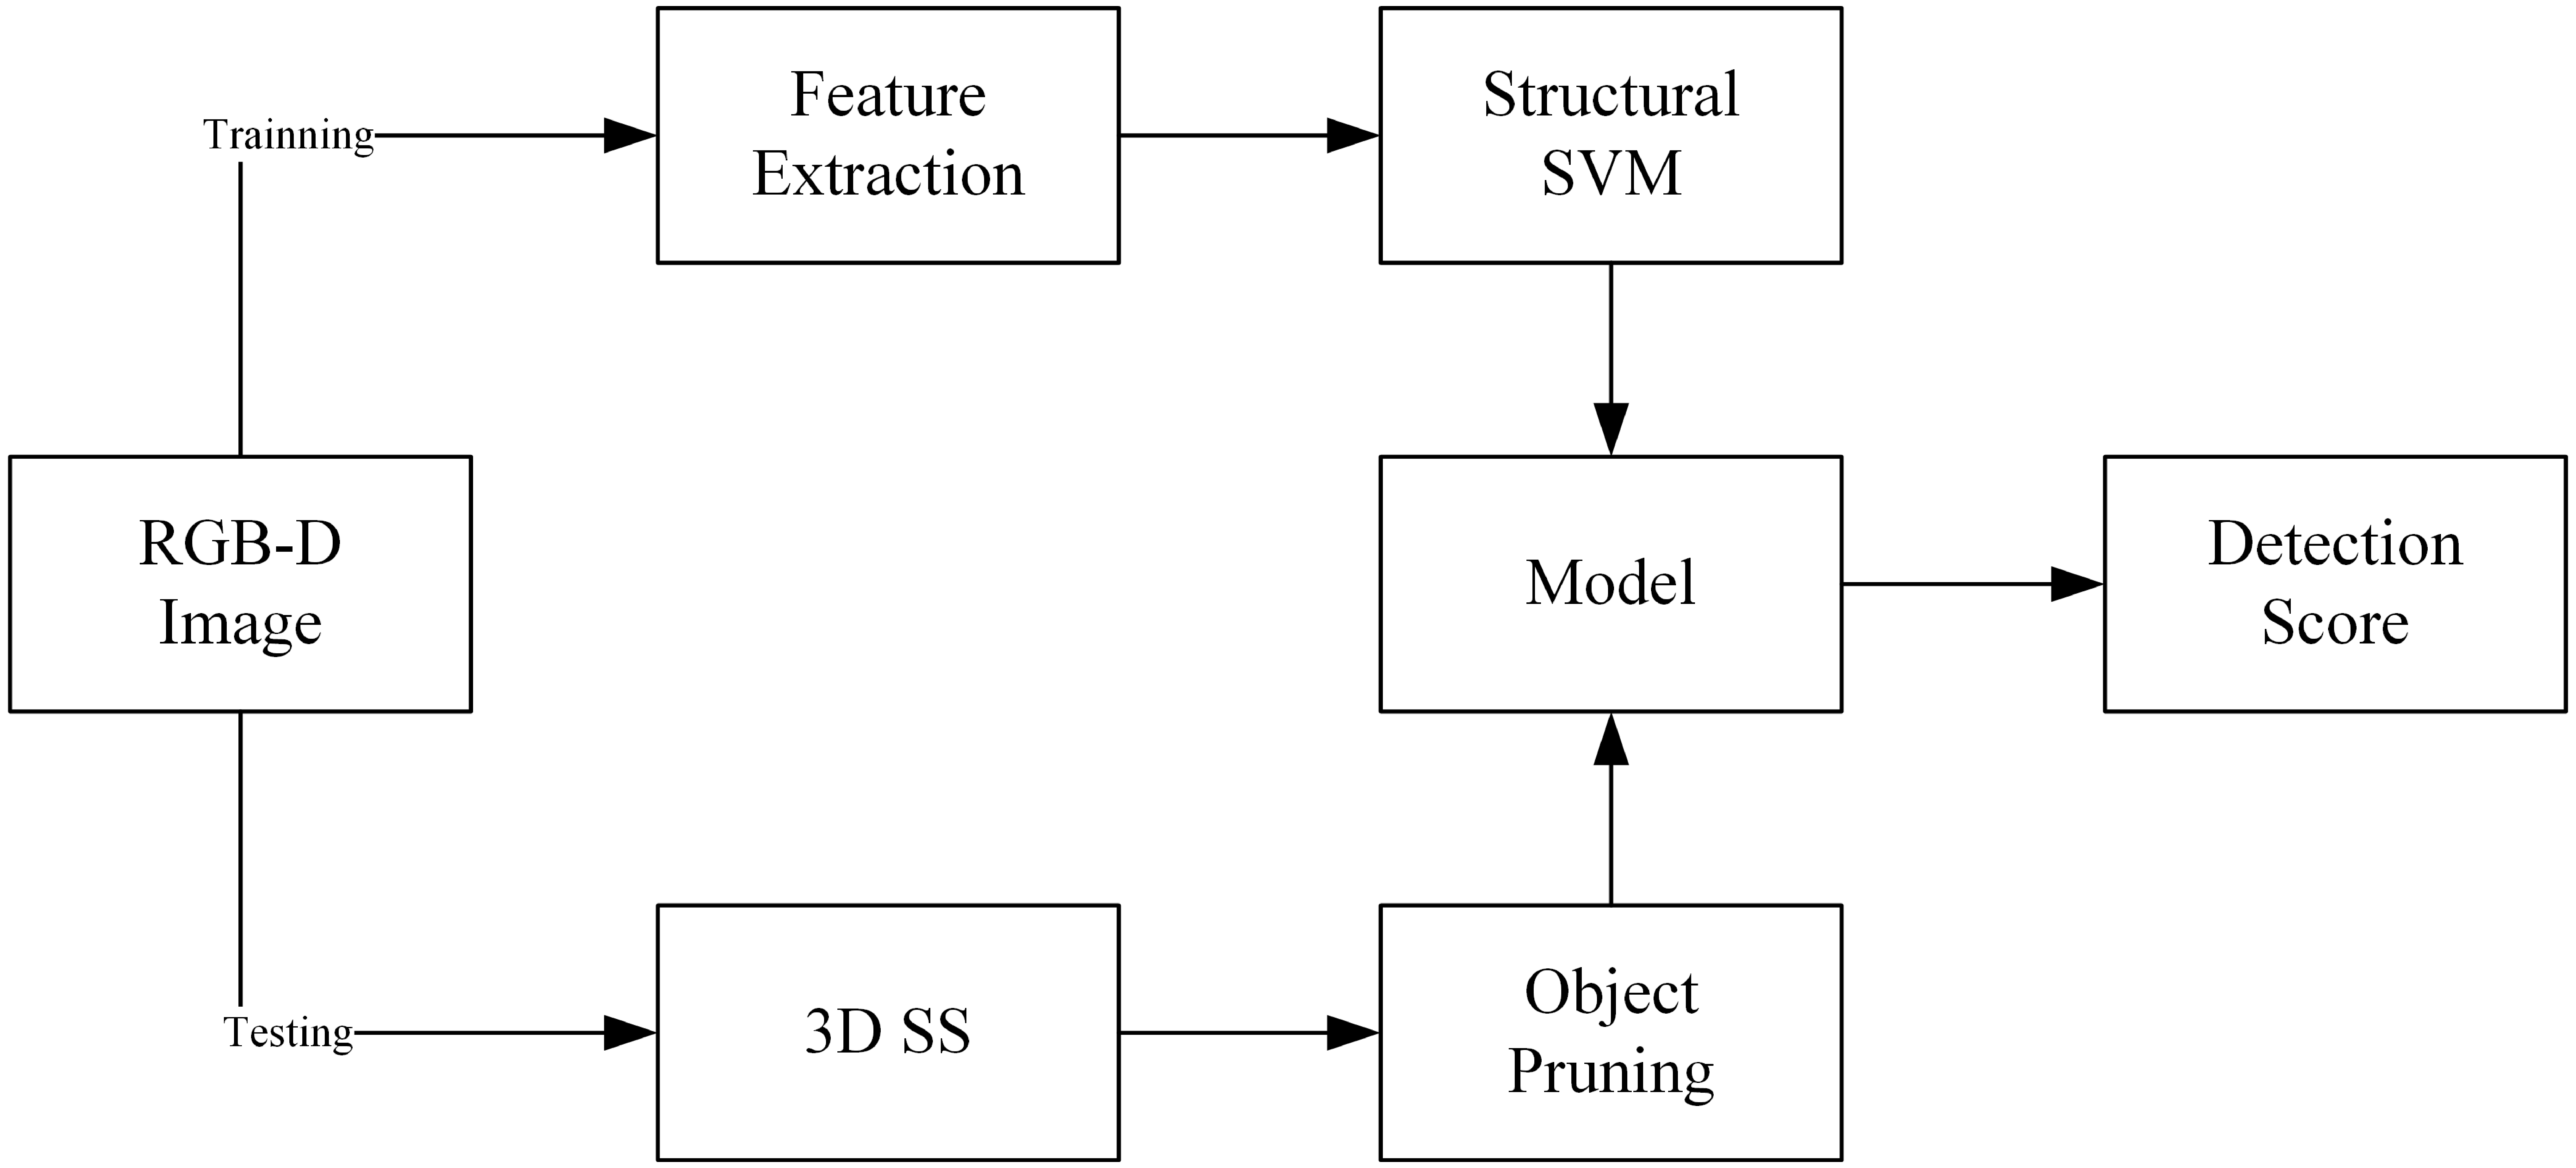
\includegraphics[width=\hsize]{3/pipeline.eps}
  \caption{whole pipeline of our detection process.}
  \label{pipeline}
\end{figure}
\subsection{Trainning}
\label{Train}
Our goal is, given certain categroy, to learn a prediction function which maps an RGBD image $I$ to a 3D cuboid $B=(L,\theta,S)$. $L$ refers to the cuboid center, $\theta$ is the cuboid orientation, and $S$ is the physical size(length, width, height) of the cuboid.
For each voxel $l$ in cuboid $B_i$ annotated in trainning image $I_i$, we have the COG feature $\phi_{il}^a$, point cloud density feature $\phi_{il}^b$, and normal histogram feature $\phi_{il}^c$. Thus the feature of cuboid $i$ is $\phi(I_i, B_i)=\{\phi_{il}^a, \phi_{il}^b, \phi_{il}^c\}_{l=1}^{216}$. \\
Given $n$ trainning examples of category $c$, we train a structural SVM\cite{joachims2009cutting} as in \cite{ren2016three} with margin rescaling constraints:
\begin{equation}
\begin{aligned}
	\min_{\omega_c, \xi_i \geq 0} \quad
	\frac{1}{2} \omega_c^\mathrm{T} \omega_c + \frac{C}{n}\sum_{i=1}^{n} \xi_i \quad \textrm{subject to}\\
	\omega_c^\mathrm{T}[\phi(I_i,B_i)-\phi(I_i, \bar{B_i})] \geq \Delta (B_i, \bar{B_i}) - \xi_i,\\
	\textrm{for all} \, \bar{B_i} \in \beta_i , i=1,...,n.
\end{aligned}
\end{equation} 
$\phi(I_i, B_i)$ are the features for 3D bounding box $B_i$ in the given RGBD image $I_i$. $B_i$ is the ground truth annotated bounding box, and $\beta_i$ is the set of candidate bounding boxes. If multiple instances are in the same image, we add images to the trainning set multutiple times, each time removing the 3D points contained in other bounding boxes.
Also, we use the following loss function to describe the fitness of groundtruth cuboid $B$
and estimated cuboid $\bar{B}$:
\begin{equation}
 \Delta (B, \bar{B}) = 1 - \textrm{IOU} \left(B, \bar{B}\right) \cdot (\frac{1+\cos(\theta - \bar{\theta})}{2})
\end{equation}
$\textrm{IOU} (B, \bar{B})$ is the volume of intersection of the cuboids, divided by the volume of their 3D union. $\theta - \bar{\theta}$ is the diffrence between cuboid orientation. After trainning, we obtain the model to dscriminate wether a cuboid belongs to this categroy.
\subsection{Testing}
\label{Test}
\cite{ren2016three} search candidate cuboid exhaustively in 3D space, which is time consuming and results many false positive. In order to fast compute cuboid hypotheses in testing image, we first use 3D Selective Search mentioned in Sec. \ref{3D Search} to obtain about 2000 candidate 3D bounding boxes, then use object pruning to further select these candidates to save time for feature computation and testing.\\
When using cuboids to represent objects,  the cuboid sizes provide underlying information about the object categories. That is the main motivation to use object pruning. First, we precompute the distribution of phisical size along each direction, aspect ratio of each pair of cuboid edge, and the centroid above ground for category $c$. Then, for each candidate cuboid, we compare these numbers with the corresponding distribution. If these values falls outside 1st to 99th percentile of the distribution, which indicate the cuboid has abnomal size, we abandon this cuboid for further testing of this catergory.\\
After object pruning, we computer the feature for prunned candidate cuboids as in trainning step. All these cuboids are evaluated use structral SVM trainned for this categroy.\\
As in \cite{song2016deep}, we use 3D Non-maximum suppression(NMS) to remove redundant bounding boxes. First, all the detected cuboids of same category are sorted based on the detection score. Then in each iteration, we select the first cuboid, with greatest detection score, and other cuboids with IOU greater than 0.35 are abandoned. At the end of iteration, we manually put the first cuboid to the last. \\
Finally, we adjust the detected bounding boxes with scaling and rotating, then find the boxes with highest score.
\section{Evaluation}
We evaluate our model on the SUN RGBD dataset\cite{song2015sun}, and compare the result with \cite{song2014sliding} and \cite{ren2016three}. We learn and evaluate appreance model of 5 object categories as in \cite{song2014sliding}. Object cuboid are generated and evaluated as described in the previous section.\\
we follow the evaluation metric in \cite{song2014sliding} with assumption that all predictions and ground truth boxes are aligned in the gravity direction. Intersection-over-union with ground-truth cuboid annotations are evaluated, and candidate boxes with score above 0.25 are consider to be correct detected. These boxes will be used to calculate the average recall for candidate cuboids generation and average precision for detection. 
\subsection{Experiments}
\begin{table}
	\centering
	\begin{tabular}{|c|c|c|c|c|c|}
	\hhline 
	&bed  &table  &sofa  &chair  &toilet  \\ 
	\hline 
	Sliding-Shape&  &  &  &  &  \\ 
	\hline 
	Geom&  &  &  &  &  \\ 
	\hline 
	Geom+COG&  &  &  &  &  \\ 
	\hline
	Ours& & & & &\\
	\hline 
	\end{tabular} 
\end{table}
\section{CONCULUSION}

%
\begin{table}
  \centering
  \caption{Font Settings}
  \label{tab2}
  \begin{tabular}{c|c}
    \hhline
    Title           & Times New Roman, 16pt,bold \\ \hline
    Author List         & Times New Roman, 11pt \\ \hline
    Authors�� Address       & 9pt \\ \hline
    Abstract, Key Words     & 9pt \\ \hline
    Section Titles      & 11pt,bold \\ \hline
    Subsection Titles       & 10pt,bold \\ \hline
    Normal Text         & 10pt \\ \hline
    Table/Figure Captions   & 9pt \\ \hline
    References, Footnotes   & 8pt \\
    \hhline
  \end{tabular}
\end{table}
%


\bibliographystyle{ieeetr}
\bibliography{pol}

\end{document}
